\documentclass[a0,portrait]{a0poster}
\usepackage{abll-poster}

\usepackage{multicol}
\usepackage{nonfloat}
\setlength{\columnsep}{88pt}


\definecolor{Shade}{HTML}{F2E6CE}


\newcommand{\Ca}{C$_{\alpha}${}}


\begin{document}
\ULCornerWallPaper{1.0}{ku-background.pdf}
\fontsize{40pt}{60pt}\selectfont

\begin{textblock}{100}(0,0)
\Faculty{\an{department of computer science}}
\\[1cm]
\Department{\an{university of copenhagen}}
\end{textblock}

\begin{textblock}{100}(0,6)
\Title{Fitting an All-atom Protein Model to a $C_\alpha$-trace}
\end{textblock}

\begin{textblock}{100}(0,13.5)
\Authors{Martin Dybdal, Anders Boesen Lindbo Larsen and Esben Skaarup}
\\[-8mm]
\AuthorEmails{\texttt{dybber@dybber.dk}, \texttt{abll@diku.dk} and \texttt{sben@diku.dk}}
\end{textblock}

\linespread{1.075}\fontsize{28pt}{40pt}\selectfont

\begin{GridBlock}{0}{21}{48}
  \Head{Motivation}
    \begin{itemize}
    \item[-- ] Proteins are the perhaps most important molecules of
      living organisms.
    \item[-- ] Computational resolution of the protein 3D-structure has
      many applications in biotechnology and medicine.
    \item[-- ] Protein structure prediction and the related topic protein
      folding, are large and active research fields.
    \end{itemize}
\end{GridBlock}

\begin{GridBlock}{51}{21}{48}
\Head{Our problem}
Nice graphics here
\end{GridBlock}

\begin{GridBlockFill}{0}{37.5}{100}

\renewcommand{\labelitemi}{--\ }

  \begin{multicols}{2}
\begin{minipage}{\linewidth} 
    \begin{multicols}{2}
    \Head{Protein Geometry}

    \begin{itemize}
    \item Proteins are built from unbranched chains of amino acids.
    \item All amino acids share
      the same basic structure and a variable side-chain.
    \item The structure of an amino acid can be described by bond lengths,
      bond angles and rotational angles.
    \item The bond lengths and bond angles only displays small variations
      between amino acids (see tables)
    \item Only three different rotational angles occurs along an amino
      acid chain. These are named $\phi$, $\psi$ and $\omega$ and are
      shown on Figure \ref{fig:torsion_angles}.
    \end{itemize} 
   \end{multicols}


\begin{multicols}{2}


\begin{minipage}{\linewidth} 
\centering

  \vspace{7mm}
  \begin{tabular}{lrr}
    \multicolumn{1}{c}{Bond} & \multicolumn{1}{c}{Avg. length} & \multicolumn{1}{c}{Std.dev.} \\ \midrule
    CA-C  & 1.5272 Å & 0.0191 Å\\
    N-CA  & 1.4680 Å & 0.0237 Å\\
    C-N   & 1.3234 Å & 0.0215 Å\\
    CA-HA & 1.0747 Å & 0.0307 Å\\
  \end{tabular}
  \vspace{4mm}
  \label{tab:average_bond_lengths}
  \tabcaption{Average bond lengths (in ångstrøm)}
\end{minipage}


\begin{minipage}{\linewidth} 
\centering
  \vspace{7mm}
  \begin{tabular}{lrr}
    \multicolumn{1}{c}{Bond} & \multicolumn{1}{c}{Avg. angle} & \multicolumn{1}{c}{Std.dev.} \\ \midrule 
    H-N-CA & 118.9553$^\circ$ & 1.9979$^\circ$\\
    N-CA-C & 110.6099$^\circ$ & 2.4668$^\circ$\\
    CA-C-N & 116.7804$^\circ$ & 1.7682$^\circ$\\
    C-N-CA & 121.4547$^\circ$ & 1.9946$^\circ$\\
  \end{tabular}
  \vspace{4mm}
  \label{tab:average_bond_lengths}
  \tabcaption{Average bond lengths (in ångstrøm)}
\end{minipage}

   \end{multicols}
\end{minipage}

\pagebreak
    
\begin{minipage}{\linewidth} 
\centering% 
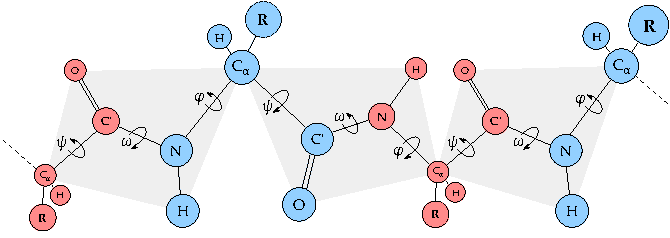
\includegraphics[width=0.90\linewidth, clip=]{../rapport/figures/protein-torsion-angles.pdf}

\figcaption{Rotational angles in a protein backbone}% 
\label{fig:torsion_angles}
\end{minipage}

\begin{multicols}{2}
  \begin{itemize}
  \item The $\omega$-angle is almost always at $180^{\circ}$, except
    for occurences where it is $0^{\circ}$. We assume that it is
    always locked at $180^{\circ}$.
  \item The $\phi$ and $\psi$ angles are the most variable parts of
    the protein backbone and many models use these as the only
    parameters when performing protein structure prediction.
  \item 
  \end{itemize}
\end{multicols}
\end{multicols}



\end{GridBlockFill}

\begin{GridBlock}{0}{75}{48}
\Head{Backbone fitting}
\textit{Bond lengths} are the distances between the covalently bonded atoms
in a molecule (usually measured in ångstrøm). We will name the
individual bond lengths by the name of the two atoms which the bond
connects. For example, the bond between a \Ca\ and N atom in an amino acid of
the protein backbone is called \Ca -N. We have computed bond lengths
for all bonds in the backbone, the results are shown in Table
\ref{tab:average_bond_lengths}. As can be seen from the last column in
the table, the variation is very limited and we therefore have not
found it necessary to consider any variations from the mean
lengths.
\end{GridBlock}

\begin{GridBlock}{51}{75}{48}
\begin{wrapfigure}{r}{0.55\textwidth}
    \centering
    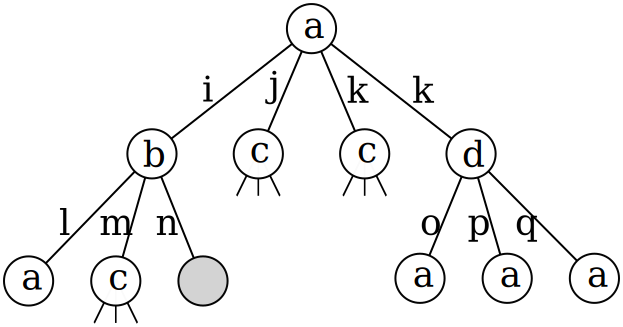
\includegraphics[width=.45\textwidth]{../rapport/figures/rotamersearch}
    \caption{The structure of our rotamer search space when
      eliminating collisions with the amino acid \textit{a}.}
    \label{fig:rotamer-search-tree}
\end{wrapfigure}
\Head{Rotamer selection}
\textit{Bond lengths} are the distances between the covalently bonded atoms
in a molecule (usually measured in ångstrøm). We will name the
individual bond lengths by the name of the two atoms which the bond
connects. For example, the bond between a \Ca\ and N atom in an amino acid of
the protein backbone is called \Ca -N. We have computed bond lengths
for all bonds in the backbone, the results are shown in Table
\end{GridBlock}

%\begin{GridBlock}{51}{80}{48}
%\Head{Conclusion}
%\begin{itemize}
%\item[-- ] We can obtain a RMSD of less than $0.2$ Å with our devised
%  variant of cyclic coordinate descent
%\item[-- ] Selecting the appropriate rotamers makes it possible to
%  reduce the number collisions to 1 for every 4700 amino acids on a
%  realistic protein.
%\end{itemize}
%\end{GridBlock}


% If you want to add a figure do something like this:




\end{document}

